\chapter{RF Fundamentals}\label{fundamentals}

\minitoc 

\clearpage
\section*{Objectives}
To develop a sound, practical understanding of:
\begin{itemize}

\item radio frequency behaviour (propagation characteristics, frequency band selection and range);

\item the variation in the relationship between power and distance for different frequencies;

\item impact of Interference (sources of noise and interference);

\item antenna systems (type selection);

\item channel bandwidth (vs frequency bands);

\item the Shannons-Hartley law
 
\item system gain; 

\item reflection and refraction of wireless signals.

\end{itemize}


\section{Wireless Signal Characteristics}

\subsection{Power vs distance}

The power of an electromagnetic signal reduces over distance because,
as the signal propagates through space, the energy it carries is spread
over a larger area. This is illustrated in Figure \ref{inversesquarelaw}.
\begin{figure}
	\centering
	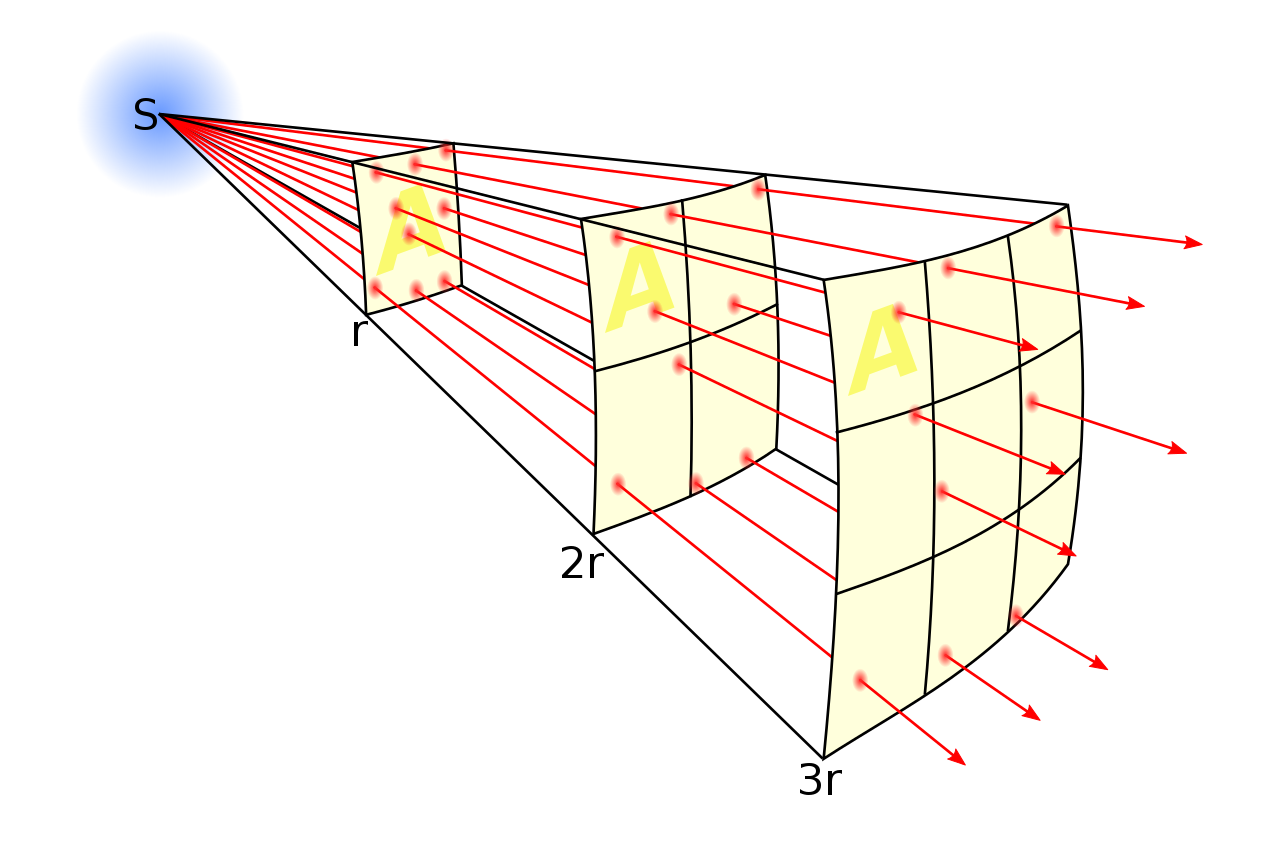
\includegraphics[width=10cm]{Inverse_square_law_svg}
	\caption{The inverse square law (By Borb, CC BY-SA 3.0, https://commons.wikimedia.org/w/index.php?curid=3816716)}
	\label{inversesquarelaw}
\end{figure}

In fact, from the principle illustrated in Figure \ref{inversesquarelaw}, we can conclude,
more precisely, that the power of a signal decreases in proportion to the square of the distance
between the sender and the receiver:
\begin{equation}
	P_d = \frac{1}{d^2} P_1,
\end{equation}
in which $P_d$ denotes the power of the signal received at distance $d$ from the transmitter.

This assumes that the signal is not absorbed by the medium; for example, if the space between
the sending antenna and the receiving antenna is completely empty -- a vacuum -- we can expect
the inverse square law to be exact. But if the space has some contents, e.g. air, glass, water, 
mist, clouds, rain, etc, then there will be some absorption of energy in the intervening space
and the inverse square law will not hold exactly.

\subsection{Power vs Frequency }

\subsection{Noise and interference}

\section{Antenna Design and Choice}

Antenna design is tricky to explain, and to do. Fortunately,
most of us do not need to {\em design} antennas, but merely to
choose the appropriate one from a small range of alternatives, in
a certain situation. Nevertheless, there some simple principles
which we can easily learn that make it a lot easier to make these
choices correctly.

\subsection{Dipole Antennas}

\subsection{Frequency dependence}

\subsection{Reciprocity}



\section{The Shannon-Hartley law}

\section{System Gain}

\subsection{Free space loss}

\subsection{Antenna gain}

\subsection{Feeder loss}

\subsection{Transmitter power}

\subsection{Receiver sensitivity}


\section{Reflection and Refraction}


